\section{The Design of LIGNUM}

The  design of  any  computer  program includes  the  decision how  to
represent information  and concepts from the real  world. C++ supports
many   programming   methodologies   (perhaps  most   notably   object
orientation)  but  the  emergence  of the  Standard  Template  Library
emphasizes   generic   programming   with  abstract   datatypes   that
encapsulates data and algorithms  working with this data. 

Two language  constructs in C++ are  of special importance for generic
programming: classes  and   templates.   A class  defines   a datatype
consisting   a  set of   possible   states  and  operations   defining
transitions between those states. Template  is simply the C++ term for
a parameterized type.

\subsection{Units of LIGNUM} 

The main design  principle in  \lignum\ is to   model a tree with  few
simple  basic units  that correspond to   the organs of  the tree. The
units must  be   such that  they allow   a  detailed analysis  of  the
structure and the development of the tree during its life time and and
still keeping  the  model computationally manageable to  create forest
stands consisting of different tree species.  Ideally the units should
be such that they can be divided  into more detailed tree compartments
if necessary.

Currently  a tree is  modeled in  \lignum\ with  five units.   The two
basic units  (i.e., they are not  aggregates of other  units) are tree
segment (TS)  and bud (B).   Axis (A) is  an aggregate or  sequence of
tree  segments sepaterated  by  branching points  (BP)  ending with  a
terminating  bud  and models  one  single  branch  in a  tree  (Figure
\ref{fig:struct}). Branching  point is an aggregate  of axes capturing
the branching  structure of a tree.   The fifth unit  is naturally the
tree itself, an aggregate of all its tree compartments.

\begin{figure}[h]
\begin{center}
\includegraphics[width=0.8\textwidth,height=0.5\textwidth]{Lignum3D.eps}
\caption{ A model tree presented in \lignum\
(left). Cf. young Scots pine\\produced by \lignum\ (right).}\label{fig:struct}
\end{center}
\end{figure}

The main functioning unit tree segment consists of sapwood, heartwood,
bark and  foliage and it  captures the main  metabolic functiong  in a
tree.  The tree segment corresponds roughly to the annual shoot but in
the   strict modeling sense this is   not necessarily always the case,
especially when modelling heartwood trees.

The bud is  an  embryonic shoot, the  growing  point of the tree  from
which new shoots, leaves and flowers may develop.  Buds can be further
divided  into terminal buds located at  the top of  axes and lateral
(or   axillary) buds  located   in the  tree   segment.  Further,  for
heartwood trees the lateral buds are located where the leaf petiole is
attached to a tree segment.

From the modeling point of view the branching point is the place where
two or more  tree  segments are  connected  to each other.   The  axis
corresponds to a stem or a branch of a tree.

\subsection{Program Architecture}

As a tree is represented with  five units in \lignum\ a natural choice
is to represent each unit as a class.  Each unit will have its own set
of attributes  and operations.   An axis being  a dynamic  sequence of
alternating  tree   segments  and  branching  points   ending  with  a
terminating  bud can be  straightforwardly represented  by a  list.  A
common notation for a list is to denote the beginning of a list with a
left  bracket ($[$)  and the  end  of the  list with  a right  bracket
($]$). The elements  in the list are separated  by commas ($,$).  With
this formal notation the the sample tree can be now expressed as:

\begin{displaymath}
[TS,BP,TS,BP,B]
\end{displaymath}

Branching  point connects a  set of axes  in a tree.  Thus a logical
and consistent design choice is to define branching point as a list of
axes. For   example, a more  detailed structural  description of the
sample tree folds out the branching points in the main stem:

\begin{displaymath}
[TS,[A,A],TS,[A,A],B]
\end{displaymath}
 
Further more the classes for the  units of \lignum\ are organized in a
hierarchy with  a common (abstract) base  class called TreeCompartment
(TC) (Figure \ref{fig:omt} on page \pageref{fig:omt}).  This design allows
us  to  utilize polymorphism  when  implementing metabolic  processes.
Polymorphism means  that a  programming language allows  operations of
the  same  name (e.g.,  photosynthesis)  to  take  different forms  or
implementations in different units.


By defining attributes, methods and  functions that describe different
tree   compartments  one  could start   to    implement different tree
species. This is in fact how the first tree  species, Scots pine, Jack
pine and sugar  maple were implemented.   However, one of the problems
with the software used to  simulate these tree  species is that it has
proven to   be difficult  to modify.     Typically  when creating  and
validating  tree models with \lignum\    one needs to experiment   with
parameter values, different light models, metabolic processes etc. The
reason why the program has been difficult  and time consuming to adapt
for different tree species is that  the data types defined (Tree, Axis
etc.) are still concret data types.

\begin{figure}[h]
\begin{center}
\includegraphics[width=0.7\textwidth,height=0.5\textwidth]{lignum-classes.eps}
\caption{\label{fig:omt} The class hierarchy in \lignum.}
\end{center}
\end{figure}

To improve the usability of the software one more level of abstraction
is needed. Instead of concrete datatypes the tree compartments must be
defined as abstract datatypes. This means type parameterization of the
tree  compartments.   One  could   naturally  parameterize  all   tree
compartments  but so  far   the two  most important   functional  tree
compartments  are the tree  segment  and the  bud.   The axis  and the
branch whorl are  essentially containers and have  not been subject to
any modeling work per se.

The type  parameterization of the tree  segment and the  bud defines a
tree as an abstract datatype.  Each tree species is parameterized with
the structure and  function of tree segments and  buds.  As an example
suppose a modeler  wants to study the development  of Scots pine.  The
first thing to do is to create a subclass of CfTreeSegment\footnote{Cf
for Coniferous}, say  PinusSylvestrisTreeSegment.  Then if the default
methods implementing the metabolic  processes are not satisfactory the
modeler must redefine the  appropriate methods.  After the changes and
possible  additions  in the  class  PinusSylvestrisTreeSegment a  tree
modeling a Scots pine can be created simply:

\begin{center}
\tt Tree<PinusSylvestrisTreeSegment> pinus\_sylvestris;\rm
\end{center}

If also  the structure  and functioning of   the bud need  changes the
modeler creates similarly a subclass  of Bud, say  PinusSylvestrisBud,
and then creates a Scots pine tree:

\begin{center}
\tt Tree<PinusSylvestrisTreeSegment,PinusSylvestrisBud> pinus\_sylvestris;\rm
\end{center}

One could  argue  that  also axes   and  branching points  should be
abstracted too.  But so   far there has   not  been a need   to assign
metabolic   processes to  these  tree  compartments.   However, it  is
possible due to  so called  default  template parameters to add  these
tree    compartments for the class  Tree   later  without breaking the
existing programming interface.

\subsection{Algorithms and Methods}

To  complete the   design  of    \lignum\ the necessery     algorithms
implemented  either   as generic   functions     or methods must    be
identified. Naturally one must accept the fact that as in any software
development this  process is incremental and   ongoing work during the
life time of the program.

The fundemantal decision is what should be assigned as methods for the
tree compartments. Technically  all algorithms could be implemented as
methods but this is  hardly a wise decision.   It  would only lead  to
constant  changes  to  the  classes   identified  so far making   them
difficult to maintain and increase the time to learn  to use them.  As
tree compartments are created  to describe the structure  and function
of a  generic tree the design  choice  is that \it  only the metabolic
processes \rm should be assigned as methods for the tree compartments.
Other algorithms traversing the model tree passing information between
tree compartments or   quering  the  status  of the  tree  should   be
implemented as generic functions.

To decide what actually  are the  metabolic  processes depends  on the
level of detail how the tree is modeled.  Scientist considering a tree
growth on cell level views the tree differently as a scientist working
on a  forest level. \lignum\ models  a tree capturing  individual tree
segments.  Thus  the metabolic processes that can  be assigned  to the
tree  compartments are photosynthesis, respiration,  flow of water and
nutrients,  length growth, diameter growth  and  the mortality of tree
compartments.

As   the  metabolic  processes   are   assigned   to   individual tree
compartments  generic algorithms are  needed to traverse  the tree and
apply these processes   to each  compartment.   So far   all metabolic
processes can  be  applied with  one  of  the following   four generic
algorithms   or   as     their   combination:   ForEach,   Accumulate,
AccumulateDown  and PropagateUp.   As the  name   suggests ForEach and
Accumulate work   as  their counter  parts   in  STL.   AccumulateDown
traverses  the tree from the  tip of the branches to   the base of the
tree. PropagetUp does the inverse. It traverses the tree from the base
to the tip of the branches.

Finally  not all computations are well  suited or even possible within
the structural description of a  tree provided by \lignum. For example
assume that  the model  for photosynthesis is  based  on amount of PAR
(photosynthetically   active  radiation).     Many   algorithms can be
developed but to compute   the   PAR  but  in \lignum\  the    current
implementation   is based on   pairwise  comparison of tree  segments.
Perhaps  the  computations could  be  made within  \lignum\ itself but
easier way  is to create  an algorithm  (using  e.g., Accumulate) that
collects the tree  segments to a  new data structure better suited for
the algorithm and  make the computations  for the PAR there.   Another
example is the modeling work already being done. The flow of water can
be modeled  using so called  connection matrix describing how the tree
segments  are connected. This information  is  also in \lignum\ but it
always up to the  modeler to decide the  trade off between the work to
adapt the  computations to \lignum\ or  to create the  data structures
from \lignum\ and work with the familiar modeling frame work.
